\documentclass{article}

\newif\ifanswers
\answerstrue % comment out to hide answers

\usepackage{fancyhdr} % Required for custom headers
\usepackage{lastpage} % Required to determine the last page for the footer
\usepackage{extramarks} % Required for headers and footers
\usepackage[usenames,dvipsnames]{color} % Required for custom colors
\usepackage{graphicx} % Required to insert images
\usepackage{listings} % Required for insertion of code
\usepackage{courier} % Required for the courier font
\usepackage{lipsum} % Used for inserting dummy 'Lorem ipsum' text into the template
\usepackage{enumerate}
\usepackage{booktabs}
\usepackage{amsmath, amsthm, amssymb}
\usepackage{caption}
\usepackage{subcaption}
\captionsetup[table]{skip=4pt}
\usepackage{framed}
\usepackage{bm}
\usepackage{float}
\usepackage[english]{babel}

\usepackage{style}
\usepackage{xcolor}
\graphicspath{{img/}} % set of paths to search for images
\usepackage{amsmath}
\usepackage{amsfonts}
\usepackage{amssymb}
\usepackage{hyperref}

\usepackage{multirow}


\newenvironment{myitemize}
{ \begin{itemize}
		\setlength{\itemsep}{0pt}
		\setlength{\parskip}{0pt}
		\setlength{\parsep}{0pt}     }
	{ \end{itemize}                  } 


\usepackage[backend=bibtex]{biblatex}                                               
%\addbibresource{papers.bib}
\bibliography{papers.bib}

\usepackage{tikz}
\usetikzlibrary{positioning,patterns,fit}

\newcommand{\ifans}{\ifanswers \textbf{Solution: }}

% Margins
\topmargin=-0.45in
\evensidemargin=0in
\oddsidemargin=0in
\textwidth=6.5in
\textheight=9.0in
\headsep=0.25in

\linespread{1.1} % Line spacing

% Set up the header and footer
\pagestyle{fancy}
\rhead{\hmwkAuthorName} % Top left header
\lhead{\hmwkClass: \hmwkTitle} % Top center head
\lfoot{\lastxmark} % Bottom left footer
\cfoot{} % Bottom center footer
\rfoot{Page\ \thepage\ of\ \protect\pageref{LastPage}} % Bottom right footer
\renewcommand\headrulewidth{0.4pt} % Size of the header rule
\renewcommand\footrulewidth{0.4pt} % Size of the footer rule

\setlength\parindent{0pt} % Removes all indentation from paragraphs

%----------------------------------------------------------------------------------------
%	CODE INCLUSION CONFIGURATION
%----------------------------------------------------------------------------------------

\definecolor{MyDarkGreen}{rgb}{0.0,0.4,0.0} % This is the color used for comments
\lstloadlanguages{Python} % Load Perl syntax for listings, for a list of other languages supported see: ftp://ftp.tex.ac.uk/tex-archive/macros/latex/contrib/listings/listings.pdf
\lstset{language=Python, % Use Perl in this example
        frame=single, % Single frame around code
        basicstyle=\footnotesize\ttfamily, % Use small true type font
        keywordstyle=[1]\color{Blue}\bf, % Perl functions bold and blue
        keywordstyle=[2]\color{Purple}, % Perl function arguments purple
        keywordstyle=[3]\color{Blue}\underbar, % Custom functions underlined and blue
        identifierstyle=, % Nothing special about identifiers
        commentstyle=\usefont{T1}{pcr}{m}{sl}\color{MyDarkGreen}\small, % Comments small dark green courier font
        stringstyle=\color{Purple}, % Strings are purple
        showstringspaces=false, % Don't put marks in string spaces
        tabsize=5, % 5 spaces per tab
        %
        % Put standard Perl functions not included in the default language here
        morekeywords={rand},
        %
        % Put Perl function parameters here
        morekeywords=[2]{on, off, interp},
        %
        % Put user defined functions here
        morekeywords=[3]{test},
       	%
        morecomment=[l][\color{Blue}]{...}, % Line continuation (...) like blue comment
        numbers=left, % Line numbers on left
        firstnumber=1, % Line numbers start with line 1
        numberstyle=\tiny\color{Blue}, % Line numbers are blue and small
        stepnumber=5 % Line numbers go in steps of 5
}

% Creates a new command to include a perl script, the first parameter is the filename of the script (without .pl), the second parameter is the caption
\newcommand{\perlscript}[2]{
\begin{itemize}
\item[]\lstinputlisting[caption=#2,label=#1]{#1.pl}
\end{itemize}
}

%----------------------------------------------------------------------------------------
%	NAME AND CLASS SECTION
%----------------------------------------------------------------------------------------

\newcommand{\hmwkTitle}{Assignment \#2} % Assignment title
\newcommand{\hmwkClass}{CS\ 234 Winter 2019} % Course/class
\newcommand{\hmwkAuthorName}{} % Your name

%----------------------------------------------------------------------------------------
%	TITLE PAGE
%----------------------------------------------------------------------------------------

\title{
\vspace{-1in}
\textmd{\textbf{\hmwkClass:\ \hmwkTitle}}}
\author{Li Quan Khoo (SCPD)}    
\date{} % Insert date here if you want it to appear below your name

\begin{document}

\maketitle
\vspace{-.5in}

\section*{Introduction}

\section{Test Environment (5 pts)}

\begin{enumerate}
\item (\textbf{written} 5pts) By inspection, action 4 of each state has the same reward as one other action in that state, which means they can be ignored in this analysis. Where the rows are the current state $s$, the columns are the next states $s'$, and the entries are the rewards:

\begin{center}
	\begin{tabular}{| l | l | l | l | l |}  
		\hline
		  & 0    & 1    & 2    & 3    \\ \hline
		0 &  0.1 & -0.2 &  0.0 & -0.1 \\ \hline
		1 &  0.1 & -0.2 &  0.0 & -0.1 \\ \hline
		2 & -1.0 & 2.0  &  0.0 &  1.0 \\ \hline
		3 &  0.1 & -0.2 &  0.0 & -0.1 \\ \hline
	\end{tabular}
\end{center}

By inspection, the optimal sequence of states is $s_0, s_2, s_1, s_2, s_1, s_0$, with a reward sequence of $0, 2, 0, 2, 0.1$, for a total of 4.1.

Observations:
\begin{itemize}
	\item There are three non-trivial rewards in the transition matrix. Two positive, one negative.
	\item All other rewards and penalties in a state do not affect the choice of path, as no sequence of these is sufficient to cancel out a non-trivial reward in a sequence length of 5.
	\item Disregarding the starting state condition, the maximal reward in a sequence of two forms a cycle between $s_2$ and $s_1$, with reward of 2. This is easily determined by inspection. Meaning for a sequence of 4, we just run this cycle twice.
\end{itemize}

Reasoning: We follow a greedy policy. The initial $s_0$ has two non-negative actions. The self-transition results in a total reward of 0.5. $a_2$ is the shortest path that leads to $s_2$, which is where both positive non-trivial rewards originate from. Both of these high reward actions have return transitions of 0 to $s_2$ or otherwise have trivial rewards. The greedy choice is to take action $a_1$ twice from $s_2$, by returning to $s_2$ via the shortest path. Finally, when we consider the final transition in $s_1$, the only reasonable choice is the greedy one, netting us the final return of 0.1.

\end{enumerate}


\section{Q-learning (12 pts)}\label{q-learn}

\begin{enumerate}
\item (\textbf{written} 3pts) Experience replay allows for learning from the same $(s,a,s',r)$ tuple multiple times. As discussed in the lectures, Q-learning does not propagate information backwards like Monte-Carlo methods do, since the trajectory has been lost. Depending on how we minibatch the tuples, the data may be less temporally-correlated, which may also give us better convergence properties.

\item (\textbf{written} 3pts) Off-policy Q-learning with function approximation has no convergence guarantees, and using experience-replay means we are necessarily operating off-policy i.e. we are using $(s,a,s',r)$ tuples collected by running a previous policy. The target network makes sure that the target Q-function (which is supposed to be approximating the optimal Q function) doesn't change within each 'batch' during training, in order to improve the chances of the algorithm eventually converging onto the optimal Q function and hence the optimal policy.

\item (\textbf{written} 3pts) I assume the question is asking about the benefit of representing the Q-function as a as a parametric function approximator $\tilde{q}(s, \mathbf{w})$ e.g. a neural net. Here I assume $\textbf{w}$ is a finite vector in $\mathbb{R}^N$. The Q-function is a mapping $Q: S \times A \rightarrow \mathbb{R}^K$. The most obvious choice for this representation is that when even $S$ or $A$ or both are either countably infinite or uncountably infinite (continuous), the set of parameters $\textbf{w}$ is still finite, and hence is always representable in finite memory.

\item (\textbf{coding} 3pts) -code-
\end{enumerate}

\section{Linear Approximation (26 pts)}
\begin{enumerate}
\item (\textbf{written} 3pts) Since $x(s,a)$ is a one-hot vector, $\hat{q}(s,a;\textbf{w}) = \textbf{w}^Tx(s,a) = \textbf{w}_{s,a}$, which corresponds to the single 1 entry in $x$.
\begin{align*}
\textbf{w} &\leftarrow \textbf{w} + \alpha\left(r+\gamma \max_{a' \in A} \hat{q}\left(s',a'; \textbf{w} \right) - \hat{q}\left(s, a; \textbf{w} \right)\right) \nabla_{\textbf{w}}\hat{q}(s,a; \textbf{w}) \\
\textbf{w}_{s,a} &\leftarrow \textbf{w}_{s,a} + \alpha\left(r+\gamma \max_{a' \in A} \mathbf{w}_{s',a'} - \mathbf{w}_{s,a}\right) 1
\end{align*}
We can see that the above update rule becomes independent of $\hat{q}$, and so our representation becomes a table of size $|S|\times|A|$, which is represented by the vector $\textbf{w}$ of length $|S|\times|A|$. Let $\textbf{w}_{s,a} = Q(s,a) \ \forall s\in S, a\in A$ and we have the equation we need. QED.

 \item (\textbf{written} 3pts) Given: $\hat{q}(s,a;\mathbf{w})=\mathbf{w}^Tx(s,a)$
\begin{align*}
 \textbf{w} &\leftarrow \textbf{w} + \alpha\left(r+\gamma \max_{a' \in A} \hat{q}\left(s',a'; \textbf{w} \right) - \hat{q}\left(s, a; \textbf{w} \right)\right) \nabla_{\textbf{w}}\hat{q}(s,a; \textbf{w}) \\
 \textbf{w} &\leftarrow \textbf{w} + \alpha\left(r+\gamma \max_{a' \in A} \mathbf{w}^Tx(s',a') - \mathbf{w}^Tx(s,a)\right) x(s,a)
\end{align*}

 \item (\textbf{coding} 15pts) -code-
 
\item (\textbf{written} 5pts) Yes, the model converges to a final score of 4.1.
\begin{figure}[H]
	\centering
	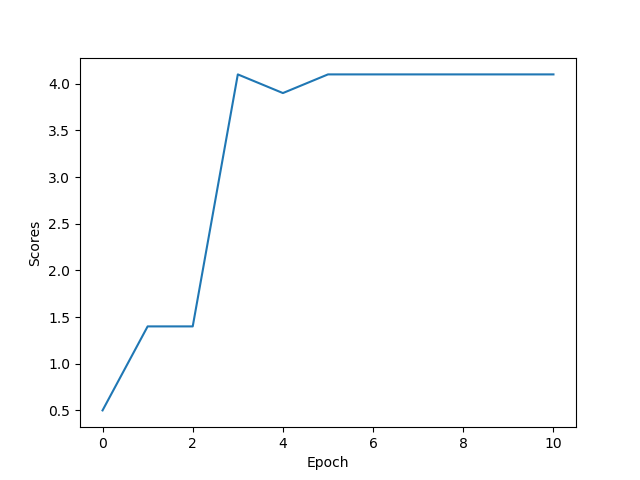
\includegraphics[width=.5\linewidth]{scores_linear}
\end{figure}

\end{enumerate}

\section{Implementing DeepMind's DQN (15 pts)}

\begin{enumerate}

\item (\textbf{coding} 10pts) -code-

\item (\textbf{written} 5pts) The models have comparable performance, but the Q-network takes longer to train.
\begin{figure}[H]
	\centering
	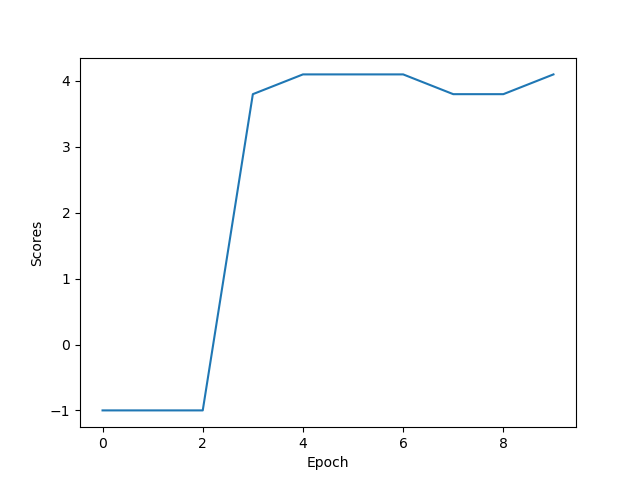
\includegraphics[width=.5\linewidth]{scores_qn}
\end{figure}

\end{enumerate}

\section{DQN on Atari (27 pts)}

\begin{enumerate}
\item (\textbf{written} 2pts) The agent requires at least 2 frames to determine the velocity of the ball. The other argument that was made by Mnih 2015 relies on the assumption that the computational load for running the emulator (environment) forward by one frame is less than computing an action for the agent. It allows the agent to observe roughly 4 times as many games (states) without also increasing the computational load by an equal amount. Having the agent make only a single every 4 frames should also have a negligible performance impact, since these Atari games are meant to be played by humans in the first place.

\item (\textbf{written} 5pts) The number of parameters in a conv2d layer is kernelHeight * kernelWidth * nInputChannels * nFilters + nBias, where the number of bias parameters is equal to the number of filters the layer has.

The number of parameters in an FC layer is nInput * nOutput + nBias, where the number of bias parameters is equal to the number of outputs the layer has.
\begin{center}
	\begin{tabular}{ | l | l | l |}  
		\hline
		Layer & Output shape & Parameters \\ \hline
		(input) & (80,80,4) & 0 \\ \hline
		Conv1 filters=32, kernel=8, stride=4, pad=same & (20,20,32) & 8*8*4*32+32 = 8192+32 \\ \hline
		Conv2 filters=64, kernel=4, stride=2, pad=same & (10,10,64) & 4*4*32*64+64 = 32768+64 \\ \hline
		Conv3 filters=64, kernel=3, stride=1, pad=same & (10,10,64) & 3*3*64*64+64 = 36864+64 \\ \hline
		FC1 & (512) & 6400*512+512 = 3276800+512 \\ \hline
		FC2 & (6) &  512*6+6 = 3072+6 \\ \hline
	\end{tabular}
\end{center}
Total = 3358374


\item (\textbf{coding and written} 5pts) The best the model did was get a max reward of -18, with mean reward of -21. This is comparable to the SARSA model in Mnih 2015, section 5.3. Perhaps this is because we are simply computing a set of 80*80*4=25600 weights for the states, the model is not expressive enough to do well, considering how large the state space actually is, even in grayscale.

\begin{figure}[H]
	\centering
	\begin{subfigure}[b]{.5\textwidth}
		\centering
		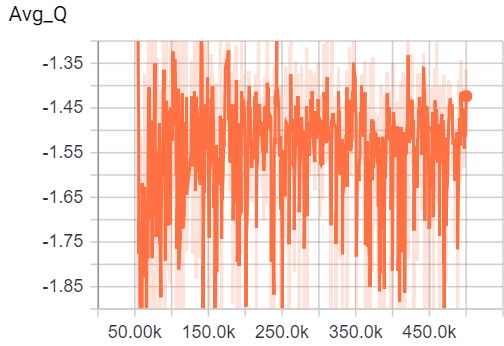
\includegraphics[width=.75\linewidth]{linear-avgq}
		\caption{Average Q}
	\end{subfigure}%
	\begin{subfigure}[b]{.5\textwidth}
		\centering
		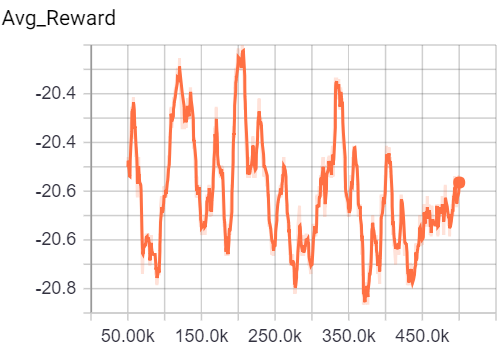
\includegraphics[width=.75\linewidth]{linear-avgr}
		\caption{Average r}
	\end{subfigure}
\end{figure}



\item (\textbf{coding and written} 10 pts)
\begin{figure}[H]
	\centering
	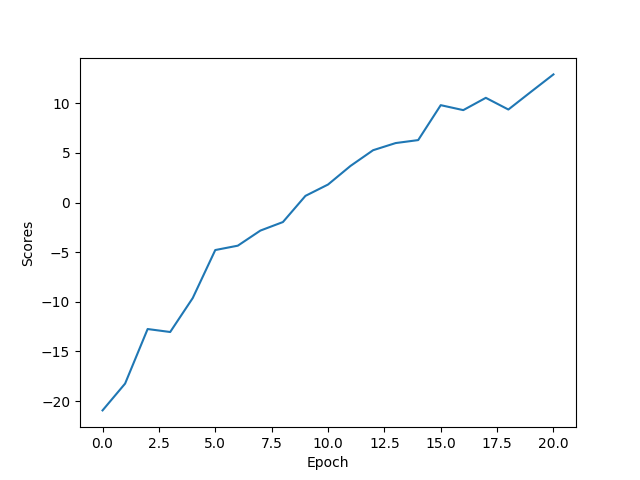
\includegraphics[width=.61\linewidth,height=5cm]{atari-scores}
	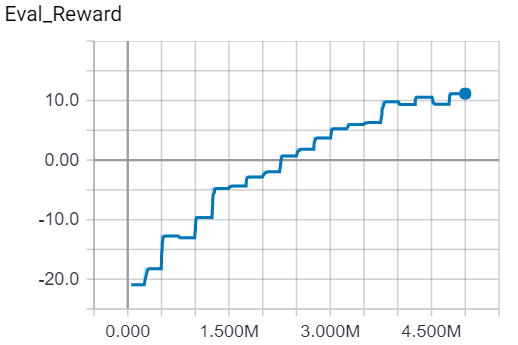
\includegraphics[width=.4\linewidth]{atari-eval-reward}
	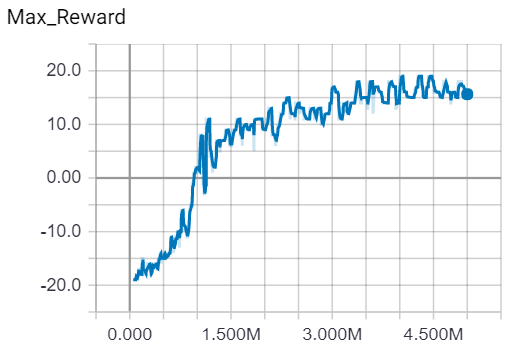
\includegraphics[width=.4\linewidth]{atari-max-reward}
	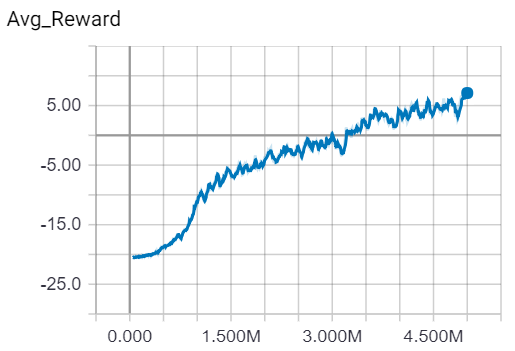
\includegraphics[width=.4\linewidth]{atari-avg-reward}
	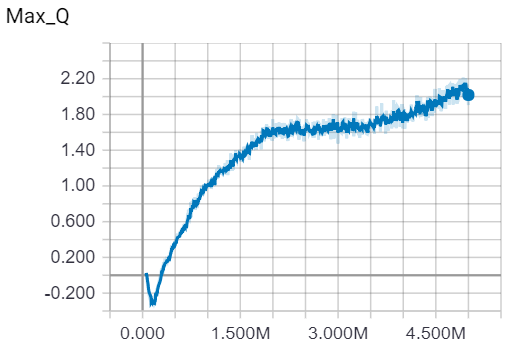
\includegraphics[width=.4\linewidth]{atari-max-q}
\end{figure}

\item (\textbf{written} 5pts) The DeepMind architecture, with its convolutional layers, is much more suited to generalizing over the possible graphical inputs. It is also a higher-capacity model, just from the number of parameters in the FC layers, so it appears to not suffer as much as the linear model from underparameterization.
\end{enumerate}

\section{Real world RL with neural networks (10 pts)}
\begin{enumerate}
\item[1.] (\textbf{written} 4pts) SGD assumes that the data we are fitting on is iid (independently and identically distributed) so that the loss function we are fitting on is stationary w.r.t the data. Since our data comes from a stream of consecutive environment interactions, this is unlikely to be the case. Depending on our choice of learning rate and choice of optimization (e.g. momentum etc) we might not converge to an optimum at all.
\item[2.] (\textbf{written} 3pts) We need to bootstrap $V(s')$, either by running our policy and taking a single-sample estimate (SARSA), i.e. $Q(s',a';\textbf{w})$, or by bootstrapping with an off-policy maximization over $Q$ (Q-learning), i.e. $max_{a'}[Q(s',a';\textbf{w})]$.
\item[3.] (\textbf{written} 3pts) Unless the state space is also finite, which brings us to the tabular case, SARSA converges under linear function approximation only, and otherwise there are no convergence guarantees.
\end{enumerate}

\end{document}
